\documentclass[../Elmag-labhefte-2020.tex]{subfiles}

\begin{document}


\setchapterpreamble[u]{\margintoc}
\chapter{The Lorentz force\label{ch.lorentz}}

\subsection*{Goal}

In this lab assignment you will
%
\begin{itemize}
    \item document experiments in the lab journal,
    \item perform error analysis of the experiment,
    \item use numerical methods to model the experiment,
    \item study forces on electrons in homogeneous and constant electric and magnetic fields,
    \item determine the ratio $e/m$ between the charge of the electron $e$ and the mass $m$ (the Thomson experiment).
\end{itemize}
%

%**********************************************
\section{Theoretical background}
%**********************************************

The theory is presented for the presentation of the calculation tasks below. Reference is also made to the textbook and the lectures in electromagnetism.

%%%%%%%%%%%%%%%%%%%%%%%%%%%%%%%%%%%%%%%%%%%%%%%%%%%
\section{Calculation tasks \label{ch.lorentz.beregn}}
%%%%%%%%%%%%%%%%%%%%%%%%%%%%%

\subsection{The Lorentz force}
%**********************************************

The force from electric and magnetic fields on charged particles is often called the Lorentz force. The force on a charged particle with charge $q$ moving at velocity $\vec{v}$ in an electrostatic field $\va*{E}$ and a magnetostatic field $\va*{B}$ is given by
\begin{equation}
    \va*{F} = q \va*{E} + q \va*{v} \cross \va*{B} .
    \label{eq:lorentz.lorentz} %(3)
\end{equation}
%
To create a fast electron beam, electric fields are always used to accelerate the electrons. However, the expression for Lorentz force shows that both electric and magnetic fields give rise to a force on charged particles.

{\emph 1. Explain from the expression of the Lorentz force why magnetic fields (as opposed to electric fields) can not give a charged particle increased kinetic energy.}

\subsection{Charges in an $E$-field}
%**********************************************

A homogeneous electric field is most easily set up between two parallel plate electrodes. This geometry provides an electric field $E = U_\mathrm{a}/\ell$ where $U_\mathrm{a}$ is the voltage between the plates and $\ell$ the distance between them.
A charged particle with charge $q$ and mass $m$ experiences an acceleration
\begin{equation}
    a = \frac{q E}{m} = \frac{q U_\mathrm{a}}{m\ell},
    \label{eq:lorentz.aksel}
\end{equation}
when travelling between the two plates.
This is used in sources of charged particle beams.

\begin{marginfigure}%[!h]
    %\setlength{\unitlength}{1mm}
    \vspace{-2cm}
    %\begin{picture}(60,60)(0,0)
    %\put(58.5,76){\large \sf 1}
    %\put(56,73){$\overbrace{}$}
    %\put(47,55.5){\vector(1,0){29}}
    %\put(44,54){\large \sf 2}
    %\put(55,53){\vector(1,0){28}}
    %\put(52,51){\large \sf 3}
    %\put(90,73){\vector(0,-1){20}}
    %\put(88,75){\large \sf 4}
    \centering
    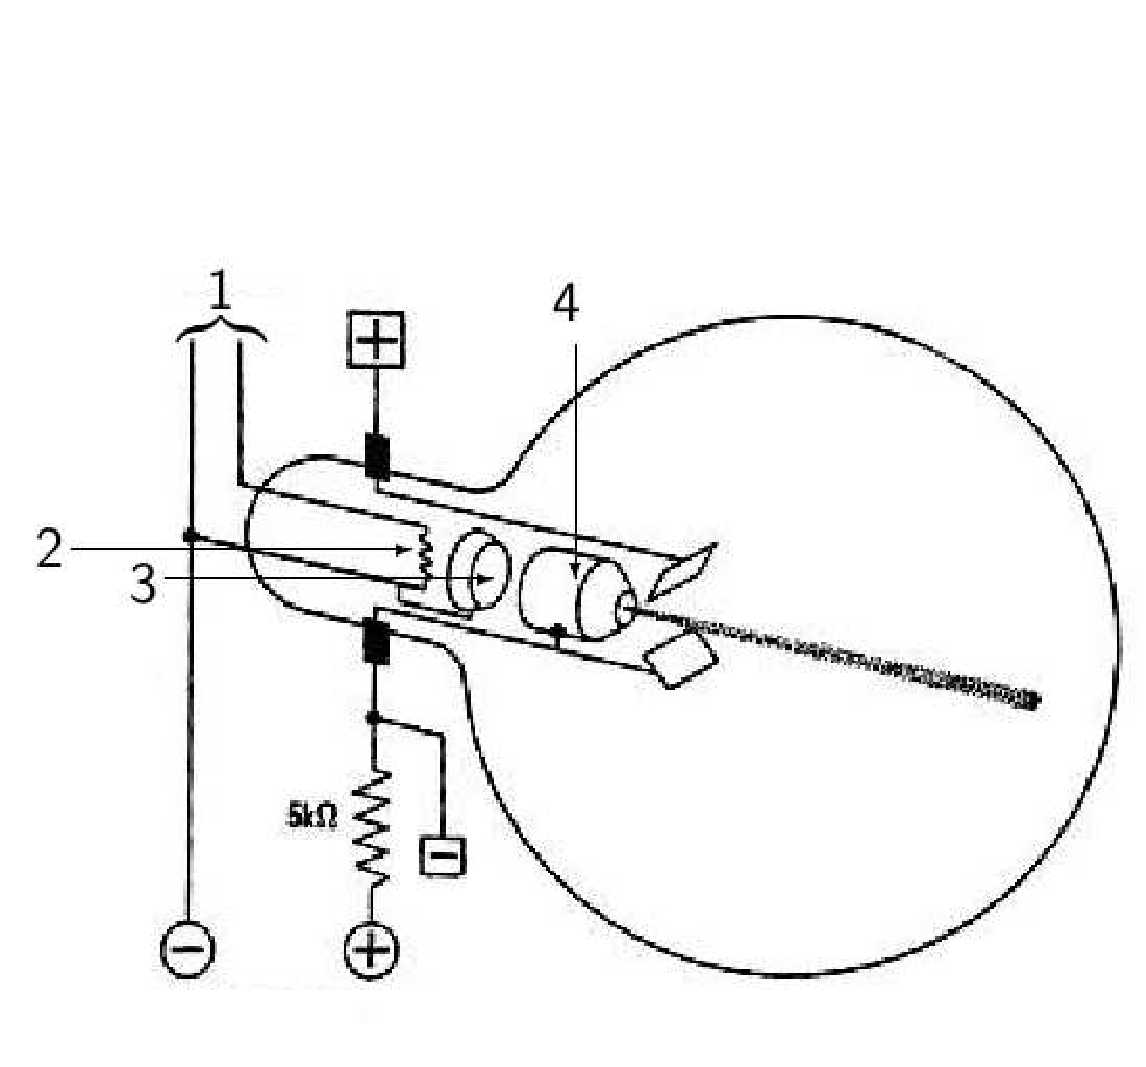
\includegraphics[width=\textwidth]{fig/LorentzFig1_resized.pdf}
    %\end{picture}
    %\vspace{-2cm}
    \caption{%
        % Prinsippskisse for elektronstrålekilde. 
        % (1) Vekselspenning (5-\SI{10}{\volt}) til 
        % (2) glødefilament varmer opp 
        % (3) oksidbelegget. 
        % Akselerasjonsspenning mellom filamentet og 
        % (4) anoden akselerer elektronene.
        Sketch of a electron beam source.
        \textbf{(1)} AC source (5-\SI{10}{\volt}).
        \textbf{(2)} Incandescent filament heats up the
        \textbf{(3)} oxide layer.
        The acceleration voltage between the filament and
        \textbf{(4)} anode accelerated the electrons.
    }
    \label{lorentz.fig1}
\end{marginfigure}
Figure \ref{lorentz.fig1} shows how an electron beam source can be made. A tungsten filament is heated by electric current passing through it. When it is red hot, it emits electrons from the surface. The filament is placed just behind a plate electrode with holes in it. Voltage is applied between the filament and the plate electrode. The electrons are accelerated towards the plate electrode and the electrons passing through the hole go out in a beam on the other side of the plate. Another way to make electrons in electron sources is to use an oxide cathode that is heated indirectly by a filament. This construction provides better field conditions during acceleration, and it is this version that is shown in Figure \ref{lorentz.fig1}.
%


Assume that an electron is accelerated from a standstill to a voltage of \SI{30}{\volt} in a static electric field.

\emph{2. What is the speed of the electron after the acceleration? }

In particle accelerator physics, the energy unit "electron volt" is abbreviated \si{\eV}. A particle with the charge \SI{1}{e} gets the energy 1 eV when it is accelerated through a voltage drop of \SI{1}{\volt}.

\emph{3A. How many joules is equivalent to \SI{1}{\eV}? }

\emph{3B. What is the energy of an electron that is accelerated to a voltage of \SI{30}{\volt} expressed in the unit \si{\eV}?}
 
An electron beam from an electron source with zero potential accelerated to a potential $U_\mathrm{a}$ can be deflected in a transverse electric field $E = U_\mathrm{d} /d$ over a distance $L$ as shown in Figure \ref{lorentz.fig2}. The deflection angle $\alpha$ is given by
\begin{equation}
    \tan \alpha = \half \frac{U_\mathrm{d}}{U_\mathrm{a}}  \frac{L}{d} .
    \label{eq:lorentz.5}
\end{equation}

\begin{figure}[!h]
    \setlength{\unitlength}{1mm}
    \begin{picture}(100,55)(20,0)
        \multiput(30,40)(2.5,0){12}{\line(1, 0){2}}%horizontal dashed
        \multiput(60,40)(4.3,0.86){14}{\line(5, 1){3.6}}%inclined dashed
        \put(60, 40){\line(1, 0){60}
        \linethickness{0.3mm}
        \put(0, -20){\line(0, 1){40}}}%screen
        %\color{red}
        \linethickness{0.1mm}
        %%%%%%%%%%%%%%%
        \put(120, 41){\Large$\downarrow$}
        \put(120, 48){\Large$\uparrow$}
        \put(121.5, 44){\line(0, 1){4}}
        \put(122, 45){\large$\Delta y$}
        \put(112, 61){\sf Screen}
        %%%%%%%%%%%%%%
        
        \qbezier(86.5,45)(88,43)(87,40)
        \put(88, 42){$\alpha$}
        %%%%%%%%%%%%%%
        \color{black}
        \put(60, 43){\line(0, 1){10}}%upper plate lead
        \put(60, 37){\line(0, -1){10}}%lower plate lead
        \linethickness{0.3mm}
        \put(53, 37){\line(1, 0){14}}%lower plate
        \put(53, 43){\line(1, 0){14}}%upper plate
        %\color{red}
        %\put(40,30){\tiny$\bullet$}
        %\put(40,50){\tiny$\bullet$}
        %\put(46,36){\tiny$\bullet$}
        %\put(46,44){\tiny$\bullet$}
        \qbezier(40,30)(43,33)(46,36)
        \qbezier(40,50)(43,47)(46,44)
        
        \put(30,35){\line(0, 1){10}}
        \put(30,35){\line(-1, 0){4}}
        \put(30,45){\line(-1, 0){4}}
        \linethickness{0.1mm}
        %%%%%%%%%
        \put(25.6,40.5){$\exists$}
        \put(25.6,36.5){$\exists$}
        \put(27.6,36.5){\line(0, 1){4}}
        \put(22,52){\sf Electron-}
        \put(22,47){\sf canon}
        %%%%%%%%%
        \put(26,36.5){\line(0, -1){13.5}}
        \put(26,23){\line(1, 0){4}}
        \put(43,33){\line(0, -1){10}}
        \put(43,23){\line(-1, 0){4}}
        %%%%%%%%%%%
        \put(30,22){$\underbrace{}_{\sf 2.0\; kV}$}
        \put(28,24){$-$}
        \put(37.5,24){$+$}
        
        \put(56,34){$-$}
        \put(56,46){$+$}
        \put(62,45.5){\sf 20\;V}
        
        %%%%%%%%%%%
        \put(52,46){\line(0, 1){8}}
        \put(51, 44){$\downarrow$}%upper plate downarrow
        \put(51, 34){$\uparrow$}%upper plate uparrow
        %\put(51, 48){$d$}
        \put(45,55){$d={\sf 2.0\; cm}$}
        \multiput(53, 36.4)(0,-2.5){6}{\line(0, -1){1}}%lower plate
        \multiput(67, 36.4)(0,-2.5){6}{\line(0, -1){1}}%lower plate
        \put(51.5,22){$\underbrace{\qquad\qquad}_{L={\sf 5.0\; cm}}$}
        %%%%%%%%%
        
        \put(90, 34.6){\vector(-1, 0){30}}%lower plate lead
        \put(90, 34.6){\vector(1, 0){30}}%lower plate lead
        \put(80,30){$L_\mathrm{s}={\sf 25\; cm}$}
    \end{picture}
    \vspace{-1.4cm}
    \caption{%
        Deflection of an electron beam in a transverse electric field.
        The numerical values in the figure are used in the exercise.
    }
    \label{lorentz.fig2}
\end{figure}

Equation \eqref{eq:lorentz.5} describes the physical laws that form the basis of the oscilloscope, which is an instrument for measuring electrical voltage. The voltage to be measured is placed between the transverse deflection plates and the deflection of the electron beam observed on a phosphorescent screen is a measure of the voltage.

%Oscilloskopet omhandles seinere i seminar i kapittel \ref{ch.oscilloskop}. Her utledes også likningen (\ref{eq:lorentz.5}), se likning (\ref{osc.6}) side \pageref{osc.6}

Assume the electrons are accelerated by a \SI{2}{\kilo\volt} acceleration potential and the other parameters are as shown in Figure \ref{lorentz.fig2}.

\emph{4. How much deflection $\Delta y$ does the beam on the screen get if the deflection voltage is \SI{20}{\volt}?}

\subsection{Charges in a \(B\)-field}
%**********************************************

When an electron moves in a space free of electric field but with a magnetic field $B$, the Lorentz force at all times acts normal to the path (unless the path is parallel to the magnetic field). Let us assume the electron is shot into the $B$-field at velocity perpendicular to the field, the Lorentz force then becomes $F_\mathrm{B} = evB$ and constitutes the centripetal force. The electron orbit becomes a circle of radius $r$ with centripetal acceleration $a_\mathrm{s} = v^2/r = F_\mathrm{B}/m$. The speed $v$ can be determined from the kinetic energy of the electron given by $\half mv^2 = e U_\mathrm{a}$. By putting these equations together, we get the following expression for the radius
\begin{equation}
    r = \frac{1}{B} \sqrt{\frac{2 U_\mathrm{a}}{e/m}} .
    \label{eq:lorentz.6}
\end{equation}

\emph{5. Set up a curve diagram curve intersections over $r$ sfa. $B$ in the range $0 < B < \SI{15}{\gauss}$ for $U_\mathrm{a} = 20$, \num{40} and \SI{60}{\volt}}. Use, for example, Python or Matlab.

\emph{5. Set up a set of curves for the radius \(r\) as a function of \(B\).}\\
Do this for the range \(B \in (\SI{0}{\gauss}, \SI{15}{\gauss})\) with \(U_{\mathrm{a}} =20, 40, \text{ and } 60\si{\volt}\).
Use for example Python or Matlab.


\subsection{Determination of \textsl{e/m} (The Thomson experiment)}
%**********************************************
 
In 1897, Thomson discovered
\sidenote{Sir Joseph John Thomson (1856--1940) was a British physicist and Nobel Laureate in Physics, credited with the discovery of the electron, the first subatomic particle to be discovered. }
%\footnote{Sir Joseph John Thomson (1856-1940), britisk fysiker. Nobelpris i fysikk 1906 for undersøkelser av elektrisk ladning i gasser.} 
extremely light, negatively charged particles -- which later turned out to be electrons. That same year, he used deflection in static electric and magnetic fields to find the relationship between their charge and mass. The expression \eqref{eq:lorentz.6} can be rewritten to
\begin{equation}
    \frac{e}{m} = \frac{2 U_\mathrm{a}} {B^2 r^2}.
    \label{eq:lorentz.7}
\end{equation}
%
The ratio $e/m$ can thus be determined by measuring the radius $r$ of the electron path of electrons accelerated by a voltage $U_{\mathrm{a}}$ in a magnetic field $B$ perpendicular to the path.

You will repeat Thomson's experiment in the laboratory. The size of the equipment limits the diameter of the largest electron orbit to approx. \SI{8}{\cm}.

\emph{6. Use the graph of the curves that you made in the problem above to estimate the appropriate magnetic field $B$ for three different acceleration voltages $U_\mathrm{a} = 20$, \num{40} and \SI{60}{\volt}.}
 
When rewriting \eqref{eq:lorentz.7} you get
\begin{equation}
    m = \frac{q B^2 r^2}{2 U_\mathrm{a}},
    \label{eq:lorentz.8}
\end{equation}
%
showing that the mass $m$ of a charged particle with a known charge $q$ that has been accelerated to a known potential $U_\mathrm{a}$ can be determined by measuring the magnetic flux density $B$ and the orbital radius $r$ of the particle in a magnetic field. This is the idea behind the magnetostatic mass spectrometer which is one of the most important instruments for determining atomic and molecular particle masses. With his work, Thomson laid the foundation for this technique.

\subsection{Voltage components \label{lorentz.spenningsdeler}}
%**********************************************
 
The so-called voltage divider is among the most common electrical connections. You must use it in the experiment. In its simplest form, the voltage divider looks like the top circuit in Figure \ref{lorentz.fig3}.

\begin{marginfigure}
  \centering
  %% We draw three diagrams that are quite similar
  %% Define the command \DefCoords which defines
  %% some key points in the diagram, making it easy
  %% to later move/change proportions.
  %%
  %% Could have been made shorter/more "programatic", but
  %% I could not be bothered.
  \newcommand{\DefCoords}{
    \coordinate (O) at (0, 0);   % Lower left corner
    \coordinate (a) at (0, 5);   % Upper left corner
    \coordinate (b) at (2, 5);   % Upper right corner
    \coordinate (I) at (2, 2.5); % "Intersection"
    \coordinate (I2) at (2, 0);  % Below intersection
    \coordinate (c) at (4, 2.5); % Corner right of intersection
    \coordinate (d) at (4, 0);   % Lower right corner
  }

  \begin{circuitikz}
    \DefCoords
    %% "Left" rectangle
    \draw (O) to[open, voltage=straight, v=\(V_{\text{in}}\)] (a) to[short, *-] (b)
    to[R=\(R_1\)] (I)
    to[R=\(R_2\)] (I2)
    to[short, -*] (O);

    %% "Right" rectangle
    \draw (I)
    to[short, -*] (c);
    \draw (I2)
    to[short, -*] (d);

    \draw (d) to[open, voltage=straight, v=\(V_{\text{out}}\)] (c);
  \end{circuitikz}

  \vspace{1cm}
  \begin{circuitikz}
    \DefCoords
    %% "Left" rectangle
    \draw (O) to[open, voltage=straight, v=\(V_{\text{in}}\)] (a) to[short, *-] (b)
    to[pR, resistors/width=2, resistors/zigs=6, n=varR] (I2)
    to[short, -*] (O);

    % Labels of var resistor
    \node[above] at (varR.wiper) {\(R_1\)};
    \node[below] at (varR.wiper) {\(R_2\)};

    %% "Right" rectangle
    \draw (varR.wiper)
    to[short, -*] (c);
    \draw (I2)
    to[short, -*] (d);

    \draw (d) to[open, voltage=straight, v=\(V_{\text{out}}\)] (c);
  \end{circuitikz}
  
  \vspace{1cm}
  \begin{circuitikz}
    \DefCoords
    %% "Left" rectangle
    \draw (O) to[open, voltage=straight, v=\(V_{\text{in}}\)] (a) to[short, *-] (b)
    to[pR, resistors/width=2, resistors/zigs=6, n=varR] (I2)
    to[short, -*] (O);

    % Labels of var resistor
    \node[above] at (varR.wiper) {\(R_1\)};
    \node[below] at (varR.wiper) {\(R_2\)};
    %% "Right" rectangle
    \draw (I)
    to[short, -*] (c);
    \draw (I2)
    to[short, -*] (d);

    \draw (d) to[open, voltage=straight, v=\(V_{\text{out}}\)] (c);

    %% The load
    \draw (c) -- ++(1.5,0) coordinate (c2);
    \draw (d) -- ++(1.5,0) coordinate (d2);
    \draw (c) -- (c2) to[R=\(R_L\)] (d2) -- (d);
  \end{circuitikz}
  \caption{Voltage dividers.
    \textbf{(Top)} With fixed resistors.
    \textbf{(Middle)} With variable resistance (potentiometer).
    \textbf{(Bottom)} With variable resistance and a load \(R_L\).}
  \label{lorentz.fig3}
\end{marginfigure}

% \begin{figure}[!ht]
% \RawFloats
%     \setlength{\unitlength}{0.75mm}
%     \begin{picture}(180,65)(-10,0)
%         \newsavebox{\ResistorSV}%Resistor Short Vertical
%         \savebox{\ResistorSV}(0,0)[l]{%
%             \multiput(14, 48)(0,-2.2){4}{\footnotesize$>$}%
%             \qbezier(14.5,50.5)(15,51)(15.5,51.5)
%             \qbezier(14.5,41.5)(15,41)(15.5,40.5)
%             \put(15.5,51.5){\line(0, 1){3.5}}
%             \put(15.5,40.5){\line(0, -1){3.5}}
%         }
%         \put(0,-4.5){\usebox{\ResistorSV}}
        
%         \put(5,4.5){\tiny$\bullet$}
%         \put(5,5){\line(1, 0){25}}%bottom line
%         \put(30,4.5){\tiny$\bullet$}
        
%         %%%%%%%%%%%
%         \put(5,54.5){\tiny$\bullet$}
%         \put(5.5,55){\line(1, 0){10}}
%         %%%%%%%%%%%%%
        
%         \put(15,29.5){\tiny$\bullet$}
%         \put(15,30){\line(1, 0){15}}
%         \put(30,29.5){\tiny$\bullet$}
%         %%%%%%%%%%%%%%%
%         %\linethickness{0.3mm}
%         \multiput(14, 48)(0,-2.2){4}{\footnotesize$>$}%
%         \qbezier(14.5,50.5)(15,51)(15.5,51.5)
%         \qbezier(14.5,41.5)(15,41)(15.5,40.5)
%         \put(15.5,51.5){\line(0, 1){3.5}}
%         \put(15.5,40.5){\line(0, -1){20}}
%         %%%%%%%%%%%%%%%
        
%         \put(5,35){\vector(0, 1){20}}
%         \put(0,30){$V_\mathrm{inn}$}
%         \put(5,25){\vector(0, -1){20}}
        
%         \put(30,20){\vector(0, 1){10}}
%         \put(30,15){$V_\mathrm{ut}$}
%         \put(30,15){\vector(0, -1){10}}
        
%         \put(18,45){$R_{1}$}
%         \put(18,12){$R_{2}$}
%         %%%%%%%%%%%
%         \put(60,4.5){\tiny$\bullet$}
%         \put(60,54.5){\tiny$\bullet$}
%         \put(60,5){\line(1, 0){35}}
%         \put(60,55){\line(1, 0){15}}
        
%         \newsavebox{\ResistorLV}%Resistor Long Vertical
%         \savebox{\ResistorLV}(0,0)[l]{%
%             \multiput(14, 48)(0,-2.2){12}{\footnotesize$>$}%
%             \qbezier(14.5,50.5)(15,51)(15.5,51.5)
%             \qbezier(14.5,23.5)(15,23)(15.5,22.5)
%             \put(15.5,51.5){\line(0, 1){3.5}}
%             \put(15.5,22.5){\line(0, -1){10}}
%         }
%         \put(59.5,20){\usebox{\ResistorLV}}
%         \put(75,55){\line(0, -1){10}}
        
%         \put(95,4.5){\tiny$\bullet$}
%         \put(95,29){\tiny$\bullet$}
%         \put(79,29.5){\line(1,0){16}}
%         \put(75,28){\large$\lhd$}  %\put(75,28){\large$\longleftarrow\!\!\!-\!\!\!-\!\!\!-$}
%         \multiput(80, 23)(0,2.5){6}{\line(0, 1){1}}
%         \put(78.6,21.6){\tiny$\bigtriangledown$}
%         \put(78.6,36.7){\tiny$\bigtriangleup$}
%         \put(67,35){$R_{1}$}
%         \put(67,22){$R_{2}$}
        
%         \put(60,35){\vector(0, 1){20}}
%         \put(55,30){$V_\mathrm{inn}$}
%         \put(60,25){\vector(0, -1){20}}
        
%         \put(95,20){\vector(0, 1){10}}
%         \put(95,15){$V_\mathrm{ut}$}
%         \put(95,15){\vector(0, -1){10}}
%         %
%         %%%%%%%%%%%%%%%%%
%         %\put(115,4.5){\tiny$\bullet$}
%         %\put(115,54.5){\tiny$\bullet$}
%         %\put(115,5){\line(1, 0){30}}
%         %\put(115,55){\line(1, 0){10}}
        
%         \newsavebox{\VoltageDivider}
%         \savebox{\VoltageDivider}(0,0)[l]{
%             \put(60,4.5){\tiny$\bullet$}
%             \put(60,54.5){\tiny$\bullet$}
%             \put(60,5){\line(1, 0){35}}
%             \put(60,55){\line(1, 0){15}
%         }
        
%         \put(59.5,20){\usebox{\ResistorLV}}
%         \put(75,55){\line(0, -1){10}}
        
%         \put(95,4.5){\tiny$\bullet$}
%         \put(95,29){\tiny$\bullet$}
%         \put(79,29.5){\line(1,0){16}}
%         \put(75,28){\large$\lhd$} %\put(75,28){\large$\longleftarrow\!\!\!-\!\!\!-\!\!\!-$}
%         %\multiput(80, 23)(0,2.5){6}{\line(0, 1){1}}
%         %\put(78.6,21.6){\tiny$\bigtriangledown$}
%         %\put(78.6,36.7){\tiny$\bigtriangleup$}
%         \put(67,35){$R_{1}$}
%         \put(67,22){$R_{2}$}
        
%         \put(60,35){\vector(0, 1){20}}
%         \put(55,30){$V_\mathrm{inn}$}
%         \put(60,25){\vector(0, -1){20}}
        
%         \put(95,20){\vector(0, 1){10}}
%         \put(95,15){$V_\mathrm{ut}$}
%         \put(95,15){\vector(0, -1){10}}
%         }
        
%         \put(70,28){\usebox{\VoltageDivider}}
%         \put(159.6,0){\usebox{\ResistorSV}}
%         \put(165,5){\line(1, 0){10}}
%         \put(165,30){\line(1, 0){10}}
%         \put(175,5){\line(0, 1){5}}
%         \put(175,30){\line(0, -1){5}}
%         \put(178,15){$R_\mathrm{L}$}
%         \put(10,60){\large \sf A}
%         \put(60,60){\large \sf B}
%         \put(130,60){\large \sf C}
%     \end{picture}
%     %\vspace{-1cm}
%     \caption{%
%         Spenningsdeler. 
%         (A) Med faste motstander. 
%         (B) Med variabel motstand med midttapping (skyvemotstand/potensiometer). 
%         (C) Med potensiometer og last $R_\mathrm{L}$.}
%     \label{lorentz.fig3}
% \end{figure}
% %

%
Through the coupling, the voltage $V_\mathrm{in}$ can be reduced to $V_\mathrm{out}$. To find the size of $V_\mathrm{out}$ as a function of $V_\mathrm{in}$ you can look at the current $I$ through the resistors $R_1$ and $R_2$ which according to Ohm's is
\begin{equation}
    I = \frac{V_\mathrm{in}}{R_1 + R_2} .
\end{equation}
Use Ohm's law again on $R_2$:
\begin{equation}
    V_\mathrm{out} 
        = I  R_2 
        = \frac{R_2}{R_1 + R_2} V_\mathrm{in}.
\end{equation}
The voltage divider can be made variable by replacing $R_1$ and $R_2$ with a potentiometer, a resistor with variable resistance, as shown in the middle circuite in Figure \ref{lorentz.fig3}.
Together with a fixed voltage source, this provides an opportunity to create a cheap variable voltage source.

However, the voltage divider has a disadvantage.

\emph{7. Can you find what disadvantage? }\\
TIP: What happens to $V_\mathrm{out}$ when you start drawing power from the output? See the bottom circuit in Figure \ref{lorentz.fig3}. The resulting resistance across the parallel connection of $R_2$ and $R_\mathrm{L}$ is denoted $R_2||R_\mathrm{L}$ and is equal to $ (R_2R_\mathrm{L})/(R_2 + R_\mathrm{L})$.


%\newpage

%%%%%%%%%%%%%%%%%%%%%%%%%%%%%%%%%%%%%%%%%%%%%%%%%%%%%%%%%%%%%%%%%%%%%%%%%%%%%%
\section{Experimental \label{ch.lorentz.eksp}}
%%%%%%%%%%%%%%%%%%%%%%%%%%%%%%%%%%%%%%%%%%%%%%%%%%%%%%%%%%%%%%%%%%%%%%%%%%%%%%

%%%%%%%%%%%%%%%%%%%%%%%%%%%%%%%%%%%%%%%%%%%%%%%%%%%%%%%%%%%%%%%%%%%%%%%%%%%%%%
\subsection{Equipment}
%%%%%%%%%%%%%%%%%%%%%%%%%%%%%%%%%%%%%%%%%%%%%%%%%%%%%%%%%%%%%%%%%%%%%%%%%%%%%%

% \vspace{-4mm}
\begin{itemize}
    \item \textbf{Electron fine beam tube.} Leybold Hereaus 555 571.
      \sidenote{\url{http://www.hep.fsu.edu/~wahl/phy3802/expinfo/em/555571e.pdf}}
    \item \textbf{Power supply for accelerator and focusing electrode.} Leybold Didactics 521 651 Tube power supply 0 ... 500 V.
    
    \item \textbf{Power supply for the Helmholtz coils.} Mascot, type 719. Used as a power source.
    Range: 0- \SI{15}{\volt}, \SI{30}{\milli\ampere} - \SI{2}{\ampere}.
    \item \textbf{Multimeter for coild current.} Escort EDM168A, 3 digits, or equivalent.
    % Presisjon: 3 sifre.
    \item \textbf{Multimeter for acceleration voltage.} Escort EDM168A, 3 digits, or equivalent.
    % Presisjon: 3 sifre.
   
    \item \textbf{Junction box with voltage divider.}
    \item Various wires of different lengths.
\end{itemize}

\begin{marginfigure}%[ht]
  \centering
  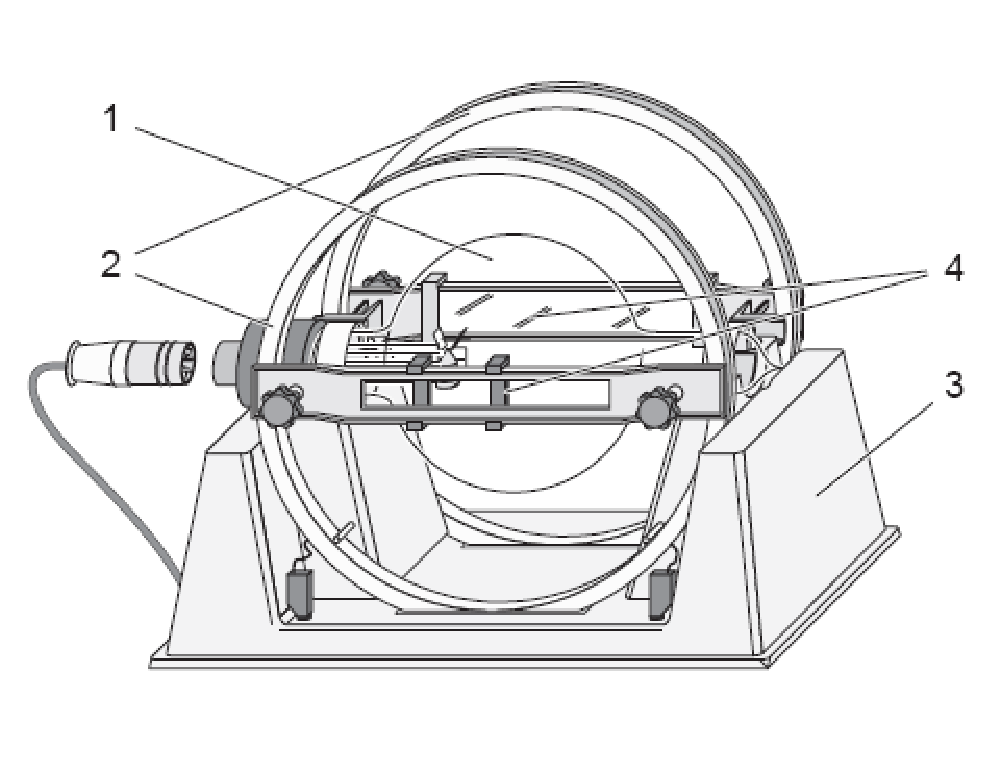
\includegraphics[scale=0.525]{fig/FineBeamApparat.eps}
  \caption{%
    The Leybold apparatus with the electron canon inside a glass vessel (1).
    Helmholtz coils (2), holder (3), and radius measuring device (4). 
  }
  \label{lorentz.fig4}
  \vspace{0.5cm}
\end{marginfigure}
\begin{marginfigure}
  \centering
  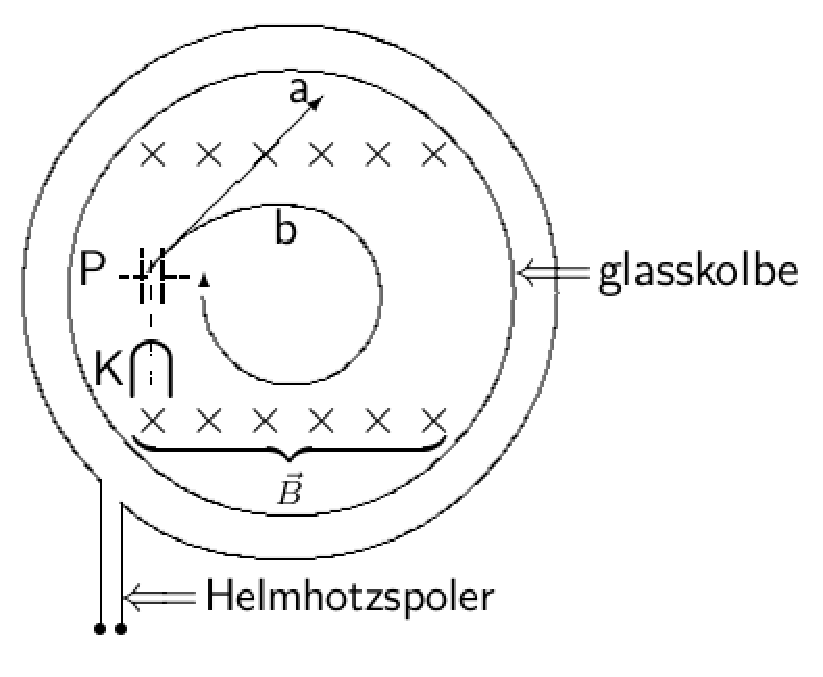
\includegraphics[scale=0.525]{fig/Schematic.eps}
  \caption{%
  Schematic drawing.
  The electron canon (K), deflection of the electron beam between the deflection plates (P).
  The magnetic field is indicated with crosses, $\times$, into the paper and the electron beam is shown without (a) and with (b) the $B$-field.}
  \label{lorentz.fig5}
\end{marginfigure}
The apparatus is shown schematically in Figures \ref{lorentz.fig4} and \ref{lorentz.fig5}. The electron gun (\textsf{K}) emits electrons that can be deflected in a static electric field between the parallel deflection plates (\textsf{P}) and/or in a static magnetic field from the Helmholtz coils. The glass flask around the electron gun is filled with thin hydrogen gas to a pressure of approximately \num{e-5} atmospheres, \SI{1}{\pascal}. Shock between the electrons and the gas will excite the electrons in the gas molecules which then relaxe and emit light (same phenomenon as in the northern lights). The trace of the electrons then becomes visible as a blue-green stripe.

\emph{Study the electron gun through the glass flask. Also study the disassembled cannon from an old beam generator laid out in the laboratory.}
\newpage
\subsection{Connection of voltages to the electron gun}
%%%%%%%%%%%%%%%%%%%%%%%%%%%%%%%%%%%%%%%%%

Figures \ref{lorentz.fig6} and \ref{lorentz.fig7} show schematically the electrical connections for the electron gun. Note the common ground point (output 2 on Leybold Power supply)

\begin{figure}[ht]
    \centering
    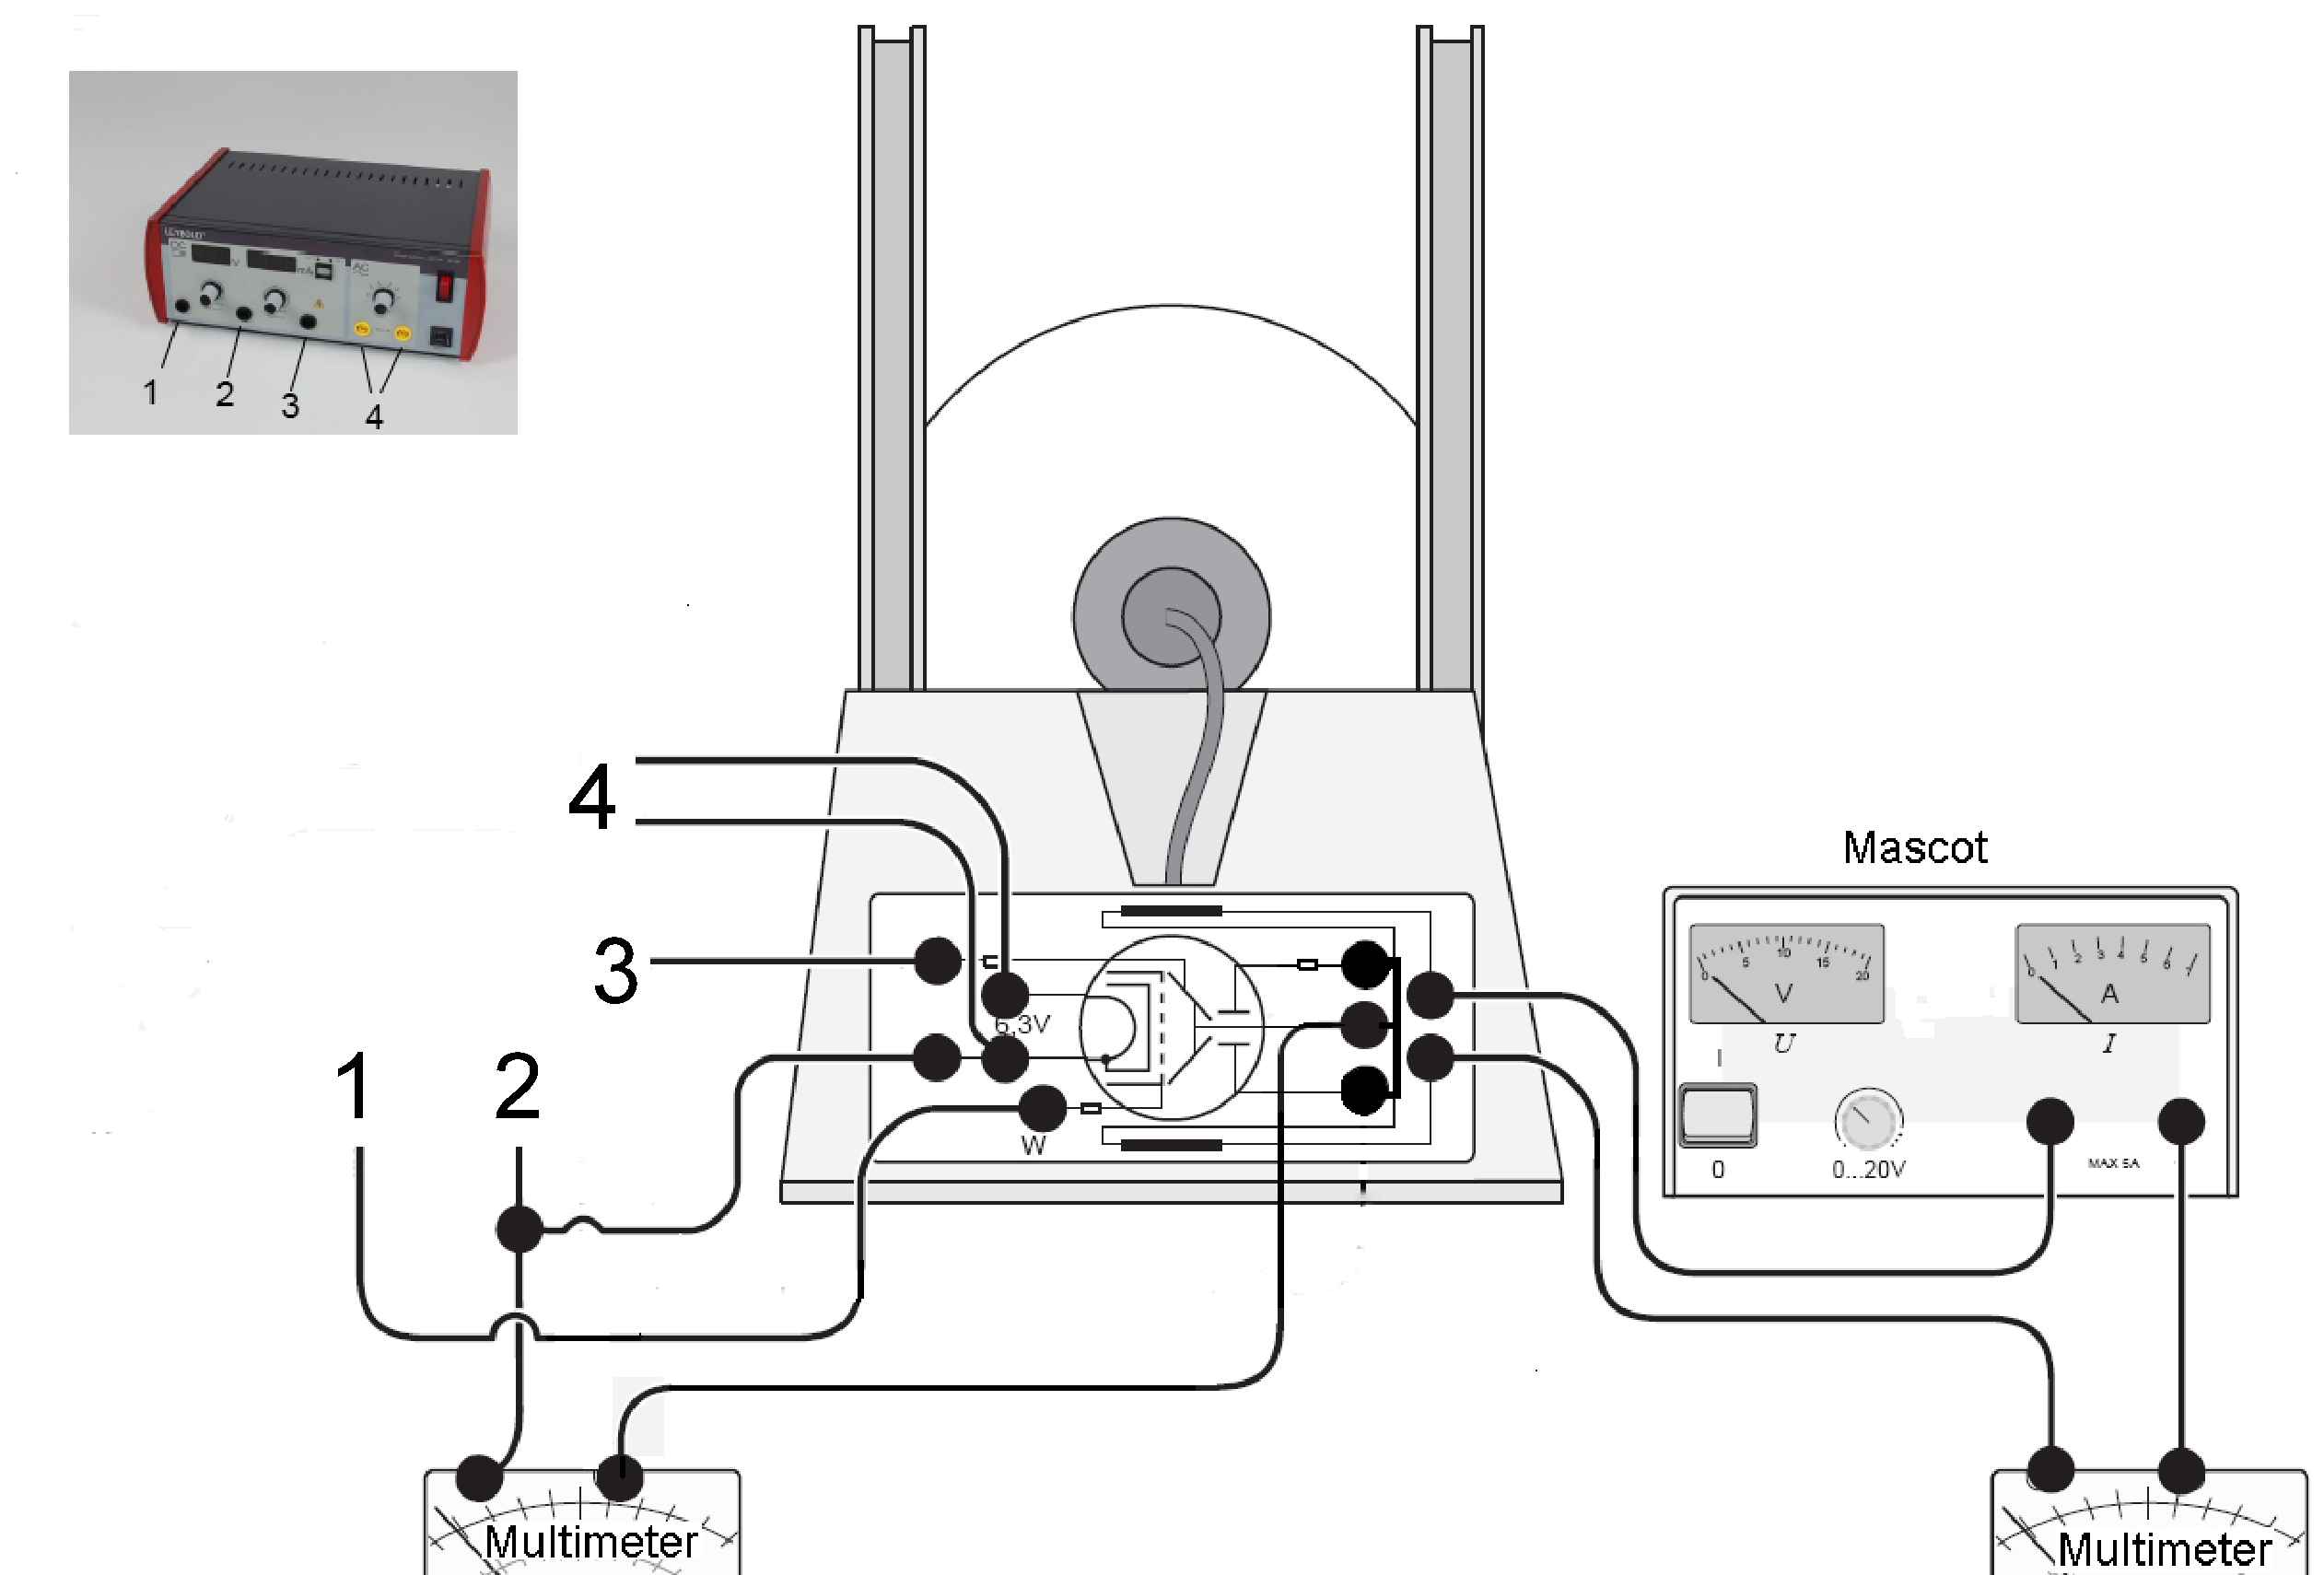
\includegraphics[width=\textwidth]{fig/Lorentz03-New.pdf}
    \caption{%
        Wiring diagram for the electron canon.
        The power supply Leybold and multimeter for measuring the anode voltage.
        See Figure \ref{lorentz.fig6} for details of the wiring diagram on the beam apparatus.
    }
    \label{lorentz.fig7}
\end{figure}

\begin{marginfigure}[-2cm]%[!ht]
  \centering
    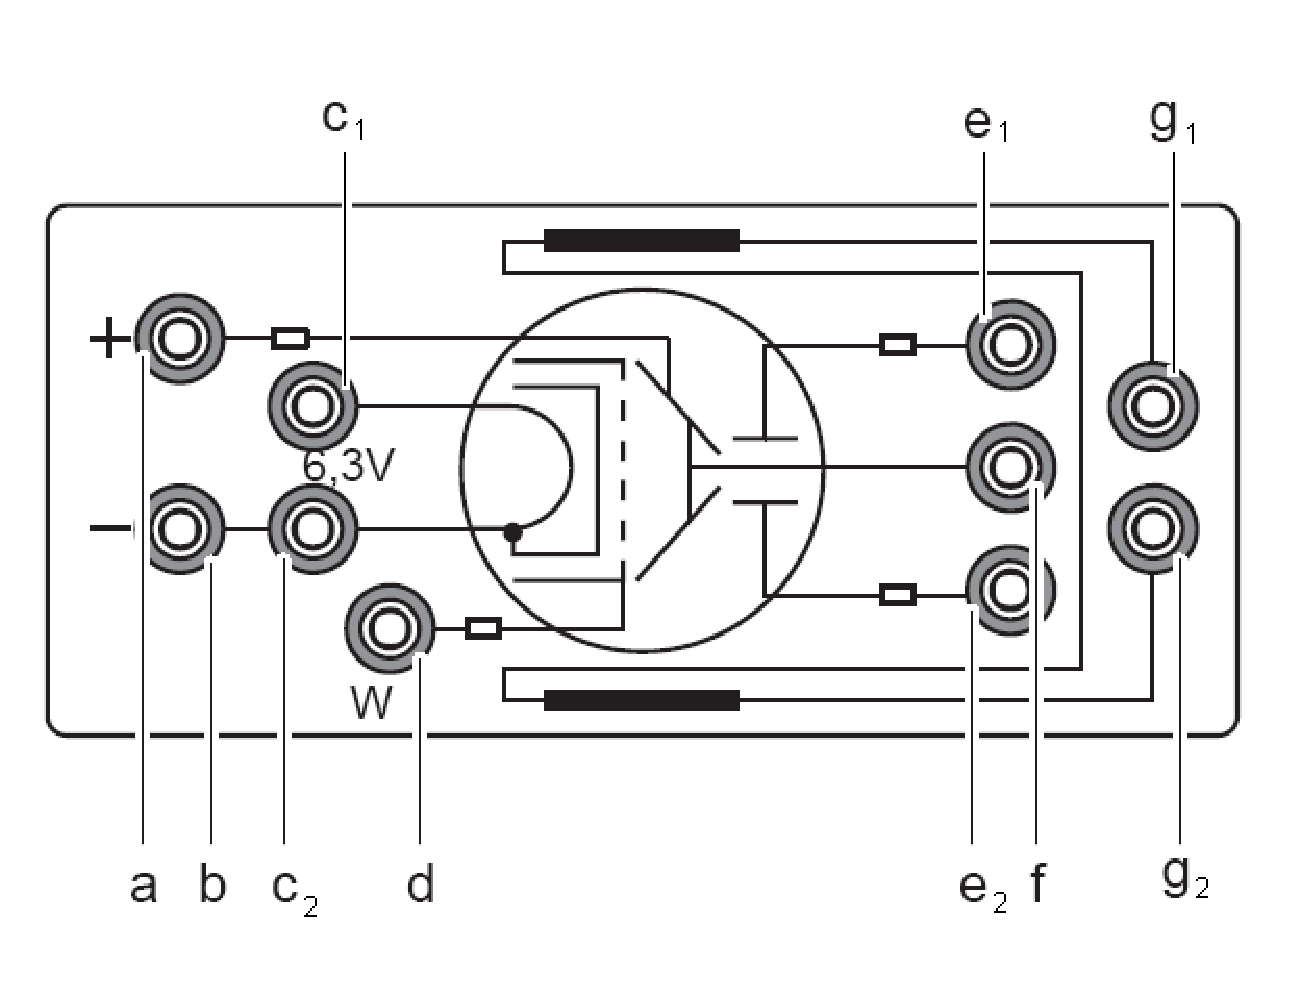
\includegraphics[width=\textwidth]{LorentzCirc0}
    % \begin{minipage}[b]{0.42\textwidth}
    %     \textsf{%
    %         a: anodespenning,\\
    %         b: jordingspunkt,\\
    %         c: glødespenning til katoden,\\
    %         d: Wehneltsylinder,\\
    %         e: avbøyningsspenning (øvre og nedre),\\
    %         f: punkt for måling anodespenning,\\
    %         g: strømtilførsel Helmholtzspoler.
    %         \vspace{15mm}
    %     }
    % \end{minipage}
    \caption{%
      Wiring diagram for the apparauts' side panel.\\
      a: Anode\\
      b: Cathode\\
      c: Cathode heating\\
      d: Wehnelt cylinder\\
      e: Deflection plates\\
      f: Anode, for symmetrical adjustment of the deflection voltage\\
      g: Helmholtz coils
    }
    \label{lorentz.fig6}
\end{marginfigure}

There are several alternative ways to connect the electron gun, but it is important to connect correctly. However, it is not difficult to break a couple of fuses if you connect incorrectly, so ask the supervisor if you are in doubt.

\emph{Connect the circuit according to figure \ref{lorentz.fig7}.}

Notes and tips:
\begin{itemize}
    \item You must connect socket 4 to the unit. Which one you use is irrelevant, but one is grounded via contacts b and c $_1$ in figure \ref{lorentz.fig6}.
    \item The unit must be switched off during connection.
    \item Ask the lab supervisor to approve the connection.
    \item Switch on the unit and adjust the glow voltage to ``6'' (V) and observe that the wire glows. This assumes that the ceiling lighting is switched off and the table lighting is dimmed. Note that the glow voltage can be lowered to 5 V during the experiments.
    \item Switch off the unit again.
\end{itemize}

%\begin{figure}[!ht]
%    \begin{center}
%    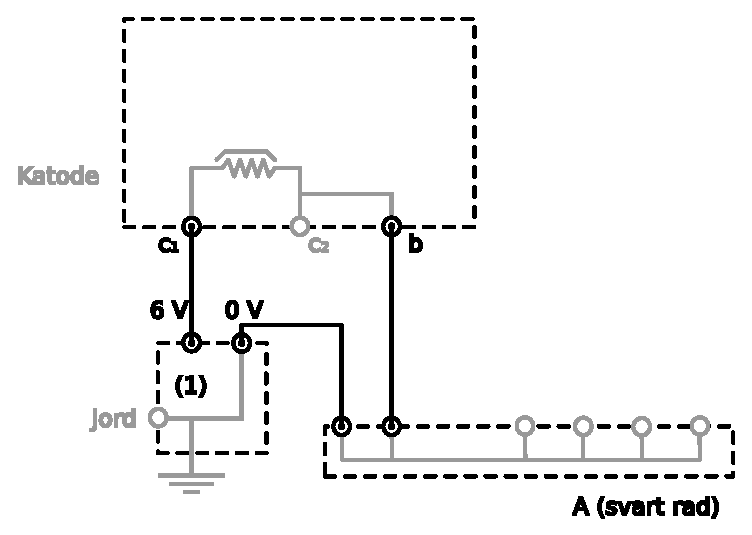
\includegraphics[width=0.6\textwidth]{glodekrets.eps}
%    \caption{%
%        Kretsdiagram for elektronkanonen, steg 1: oppkopling av glødekretsen. De delene av diagrammet som er innenfor de stiplede rektanglene illustrerer interne koplinger som du hverken kan eller trenger gjøre noe med. Bokstavene ved inngangene til elektronkanonen (det øverste stiplede rektangelet) viser til tilkoplingspunktene i figur \ref{lorentz.fig6}. Det stiplede rektangelet nede til høyre representerer den svarte raden med tilkoplingspunkter på koplingsboks A, og (1) representerer transformatoren.
%    }
%    \label{fig:glodekrets}
%    \end{center}
%\end{figure}

%\begin{figure}[!ht]
%    \begin{center}
%    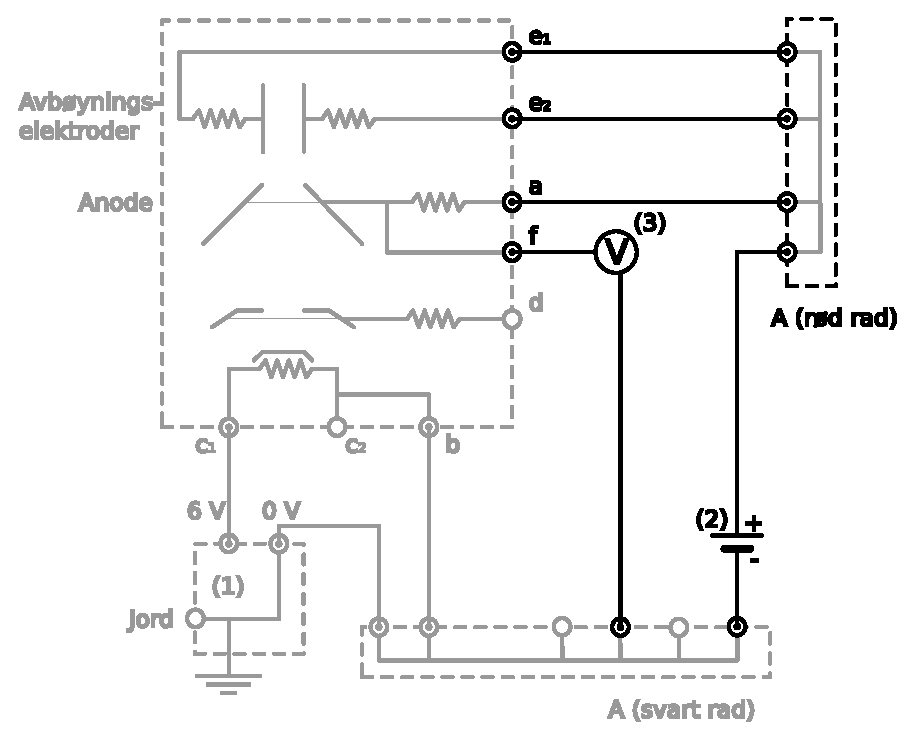
\includegraphics[width=0.6\textwidth]{anodespenning.eps}
%    \caption{%
%        Kretsdiagram for elektronkanonen, steg 2: tilkopling av anoden. De delene av diagrammet som har lysere farge er allerede oppkoplet i forrige steg; se forøvrig figur \ref{fig:glodekrets} for forklaring. Det stiplede rektangelet oppe til høyre representerer den røde raden med tilkoplingspunkter på koplingsboks A, (2) representerer Delta Elektronika kraftforsyning, og (3) representerer et multimeter for måling av anodespenning.
%    }
%    \label{fig:anodespenning}
%    \end{center}
%\end{figure}

To extract an electron beam from the cathode, the electrons must be accelerated as explained above in the theory section. This is done by applying an acceleration voltage between the cathode and the anode.

\emph{Connect the acceleration voltage according to figure \ref{lorentz.fig7}}. % og \ref{lorentz.fig7}.}

Notes and tips:
\begin{itemize}
    \item Make sure that the power supply is switched off and that the power and voltage adjustment knobs are turned all the way down when connecting.
    \item Connect Leybold output 3 to ``a'' and output 2 to ``b''.
    \item Starting potential is $U_\mathrm{d} = 0$, connect therefore the two deflection plates (e $_1$ and e $_2$) and possibly ground or connect them to the anode, to prevent charge from building up on them.
    \item To avoid measurement errors due to voltage drop across the series resistor, you can connect the voltmeter directly to the anode instead of "f". Use measuring range 1000 V DC. Check the value of the Leybold unit. How big a measurement error do you get and what determines the size of the error?
    \item The series resistors mounted internally in the equipment are inserted for safety reasons to avoid excessive current in the circuit in the event of an internal short circuit (e.g. a gas discharge).
\end{itemize}
 








%\begin{figure}[!ht]
%\begin{center}
%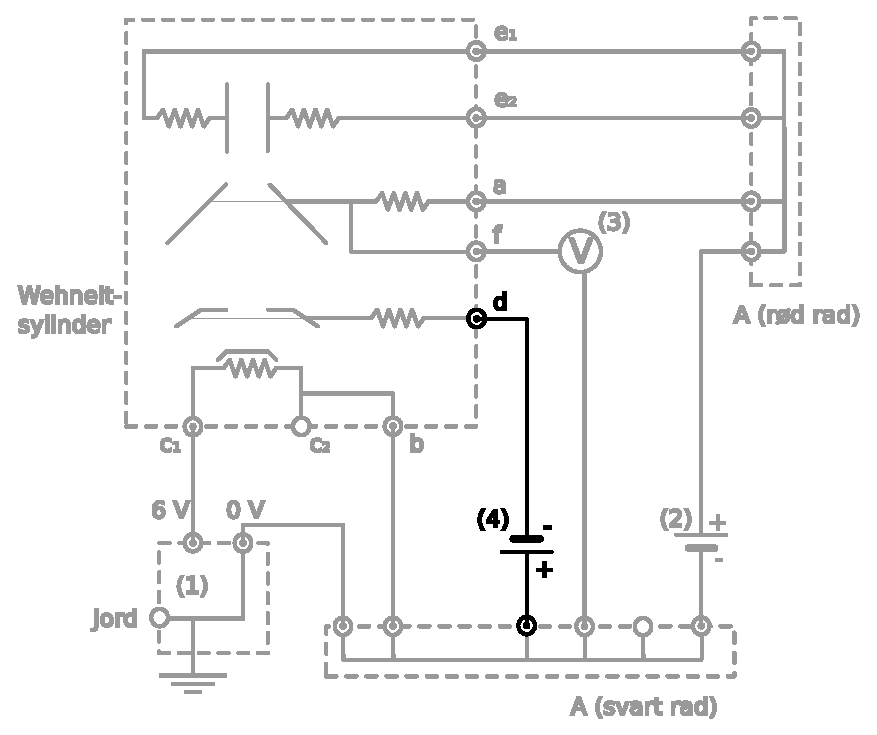
\includegraphics[width=0.6\textwidth]{fig/wehnelt.eps}
%\caption{\small\sf Kretsdiagram for elektronkanonen, steg 3: tilkopling av Wehneltsylinderen. De delene av diagrammet som har lysere farge er allerede oppkoplet i de foregående figurene; se forøvrig figur \ref{fig:glodekrets} og \ref{fig:anodespenning} for forklaring. (4) representerer en Mascot 719 kraftforsyning.}
%\label{fig:wehnelt}
%\end{center}
%\end{figure}




\emph{Now it is ready to turn on all voltages and see that the electron beam is visible:}
\begin{itemize}
\item Ask the lab supervisor to approve the connection.
\item Switch on the glow voltage.
\item Check that the filament starts to glow.
%\item Kraftforsyningen (2) for akselerasjonsspenningen skal også være spenningsstyrt: Sett METER til V, skru på og sett strømknappen 1/4 omdreining opp.
\item Increase the acceleration voltage slowly until you (at 20--30 V or slightly higher if your eyes have not adapted to the dark) see the trace of the electron beam in the hydrogen gas as a blue-violet stripe out of the electron gun.
\item Observe how the beam changes when you change the acceleration voltage.
\item Why does the beam not reach the glass wall at low acceleration? At higher voltages, quite abruptly, the beam will meet the wall, then lower the voltage slightly. This happens at different voltages at the different setups, follow closely from around 100 V, and possibly upwards to approx. 150 V.
\item NOTE: If the anode starts to glow, turn off the appliance and let it cool down. Never use higher acceleration voltages than necessary to avoid glowing.
\end{itemize}

\emph{Make a sketch of the beam path for different acceleration voltages.}
%


\emph{Procedure to turn the apparatus off:} 
\begin{itemize}
\item Switch off the glow voltage.
\item Reduce the acceleration voltage to zero and switch off the power supply.
%\item Reduser fokuseringsspenningen til null og slå kraftforsyningen av.
\end{itemize}
NOTE: It is not dangerous to have on acceleration voltage and magnetic field without having  a glow voltage, but it is not good to have on glow voltage without acceleration voltage. Therefore, always switch off the glow voltage when you have short or long breaks.

In an electron beam, all the particles have the same sign of charge. The beam will therefore have a tendency to diverge due to internal Coulomb power. If the focusing ring (Wehnelt cylinder) in front of the cathode is made slightly negative, this will have a focusing effect on the beam.

\emph{Connect the Wehnelt cylinder according to Figure \ref{lorentz.fig7}.}
Output 1 to "W".
Notes and tips:
\begin{itemize}
    \item Check that the power supply is switched off and that the power and voltage adjustment knobs are turned down completely before connecting it.
    \item After connecting the Wehnelt cylinder and switching on the power supply, adjust the voltage on the focusing electrode (Wehnelt cylinder) if you think the beam is poorly focused. Use maximum \SI{10}{\volt}.
\end{itemize}
\newpage

\subsection{Deflection in an \(E\)-field}
%%%%%%%%%%%%%%%%%%%%%%%%%%%%%%%%%%%%%%%%%

Task:
\emph{You will study the deflection of an electron beam in an electrostatic field.}

In the setup so far, you have put both deflection plates at the same voltage, namely the anode voltage $U_\mathrm{a}$. To obtain deflection, one plate is placed on a somewhat lower voltage.
This is done by adding a voltage divider to the anode voltage;
the principle of voltage division is shown in Figure \ref{lorentz.fig3}. Here you have to make changes to the connection. The anode voltage (3) should now be connected with a junction box according to the diagram in Figure \ref{fig:spenningsdeler} shows changes you must make from the connection in Figure \ref{lorentz.fig7} where the deflection potential was zero. The connection between  $e_1$ and $e_2$ is removed.
\begin{marginfigure}%[!ht]
  \centering
    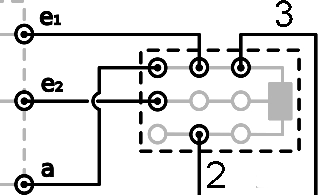
\includegraphics[width=0.9\textwidth]{fig/spenningsdeler-new.pdf}
    \caption{%
        Circuit diagram for connecting the voltage divider.
    }
    \label{fig:spenningsdeler}
\end{marginfigure}


The voltage divider consists of a precision potentiometer (Helipot) and is mounted on junction box B. The acceleration voltage $U_\mathrm{a}$ is connected across the potentiometer. From the center tapping, we take out a voltage that varies with the position of the potentiometer button, which needs 10 revolutions to turn from top to bottom. The deflection voltage is taken out between the top outlet (which is at potential $U_\mathrm{a}$) and the middle outlet at potential $x  U_\mathrm{a}$, where $x$ can vary from 0 to \SI{100}{\percent}. This means that one deflection plate is at the anode voltage $U_\mathrm{a}$ and the other at $x  U_\mathrm{a}$. The deflection voltage then becomes
\begin{equation}
    U_\mathrm{d} 
        = U_\mathrm{a} - x U_\mathrm{a} 
        = (1 - x) U_\mathrm{a}.
\end{equation}
If you connect incorrectly and take out voltage division to the ground potential, the electron beam will be reduced strongly and easily disappear. You can find out which plate should have lower potential by thinking, or by trial and error.

\emph{Connect the deflection potential according to Figure \ref{fig:spenningsdeler}.}
 

Notes and tips:
\begin{itemize}
    \item Set the potentiometer to \SI{100}{\percent} so that the center tap has the same potential as the anode voltage.
    \item Switch on glow, focusing voltage and acceleration as described previously.
    \item Vary the deflection by turning the potentiometer knob.
\end{itemize}

\emph{Explain what you observe with regard to the expression of the Lorentz force in equation \eqref{eq:lorentz.lorentz}.}

\emph{Sketch the beam for different deflection stresses, e.g. $U_\mathrm{d} = \half  U_\mathrm{a}$ and $\frac{4}{5} U_\mathrm{a}$.}


 
\subsection{Deflection in a \(B\)-field}
%%%%%%%%%%%%%%%%%%%%%%%%%%%%%%%%%%%%%%%%%

Task:
\emph{You will study the deflection of an electron beam in a static magnetic field.}


\begin{itemize}
\item Connect the equipment according to Figure \ref{lorentz.fig7}. Note that the connection of the voltage divider in the previous step is not necessary for the tests to be performed here
\item Connect the circuit to the magnets with the Mascot unit in (g).
\end{itemize}
%\begin{figure}[!ht]
%    \begin{center}
%    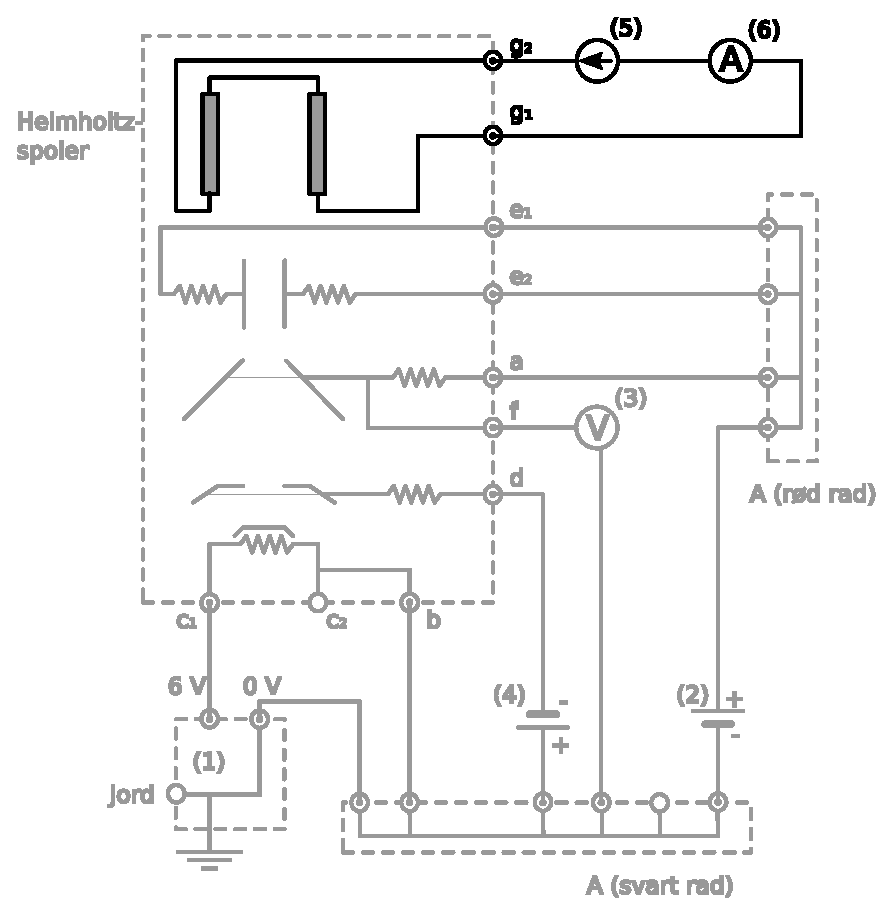
\includegraphics[width=0.6\textwidth]{fig/magnetfelt.eps}
%    \caption{%
%        Kretsdiagram for elektronkanonen, steg 5: tilkopling av Helmholtzspolene. De delene av diagrammet som har lysere farge er allerede oppkoplet i de foregående figurene; se forøvrig figur \ref{fig:glodekrets}, \ref{fig:anodespenning} og \ref{fig:wehnelt} for forklaring. 
%        (5) representerer en Mascot 719 kraftforsyning som strømkilde og 
%        (6) representerer et multimeter for måling av strømstyrken. Merk at oppkoplingen av spenningsdeleren i forrige steg (figur \ref{fig:spenningsdeler}) ikke er nødvendig for forsøkene som skal utføres her, og den er derfor ikke inkludert i dette diagrammet. Legg merke til at kretsen for Helmholtzspolene er uavhengig av resten av oppkoplingen.
%    }
%   \label{fig:magnetfelt}
%    \end{center}
%\end{figure}

Notes and tips:
\begin{itemize}
    \item Verify that the power supply for the Helmholtz coils is switched off and that the control \ buttons for current and voltage are turned down completely.
    \item Set the power supply to the power source (METER: A and the control knob for voltage up 1/2 revolution) and set RANGE to \SI{15}{\volt}.
    \item Use the multimeter (6) for current measurement.
    \item Turn up the current to approx. \SI{1}{\ampere}, and check that the circuit is working. NOTE: The coils can withstand max. \SI{2}{\ampere}. Turn the current down again afterwards.
    \item Switch on the electron beam as described earlier.
    \item Adjust the acceleration voltage to approx: \SI{100}{\volt} and the magnetic current to \SI{0.75}{\ampere}.
\end{itemize}

\emph{Explain what happens using the expression for the Lorentz force.}

Ask the lab supervisor to help you twist the electron beam tube until the beam takes a helical path.

\emph{Sketch the beam and explain the reason for the helical path.}

\subsection{The Thomson Experiment: Measurement of \(e/m\)}
%%%%%%%%%%%%%%%%%%%%%%%%%%%%%%%%%%%%%%%%%

Task:
\emph{You will find the relation \(e /m\) between the electron charge and mass from equation \eqref{eq:lorentz.7} by measuring the acceleration voltage $U_\mathrm{a}$, the radius $r$ of the electron orbit and the magnetic field $B$.}

The magnetic field is pre-calibrated against the current in the coils. The result is given in a calibration curve attached to the apparatus and as an empirical expression of the magnetic field as a function of the measured coil current found from the calibration curve. Alternatively, this expression can be used:
\begin{equation}
    B=\mu_0 \cdot \left(\frac{4}{5} \right)^{3/2}\cdot \frac{n}{R} \cdot I,
\end{equation}
with \(R\): Radius of the coils, \(n\): number of turns = 130 per coil.

Notes and tips:
\begin{itemize}
    \item Align the tube so that the beam becomes a circle and not a helix.
    \item Set the multimeter for voltage measurement in the range 0-\SI{1000}{\volt} DC voltage.
    \item Ask the lab supervisor to show you how to measure the diameter of the electron path using the parallax mirror behind the electron beam tube and a ruler.
    \item It is possible to photograph the electron path and analyze in TRACKER to get the diameter of the path. Note that you must have a scale (ruler) in the image.
\end{itemize}

\subsubsection{Analysis and Discussion of the Thomson Experiment}
%%%%%%%%%%%%%%%%%%%%%%%%%%%%%%%%%%%%%%%%%

\begin{itemize}
    \item Determine $e/m$ for the electron based on your measurements of $U_\mathrm{a}$, $r$, $I$ and the calibration curve or formula for $B(I)$.
    \item If you have time, repeat the experiment for another set of values of $U_\mathrm{a}$ and $I$.
    \item Estimate the errors in the measured quantities and find the measurement error in $e/m$.
    %\item 
    Which sources of error dominate?
    \item Compare the measured value of $e/m$ with the table value.
    \item What is the correspondence between the measurement results from different values   of $U_\mathrm{a}$ and $I$ and your error estimate?
    \item Discuss possible applications of the physical effects that have been observed in the experiment.
\end{itemize}

%%%%%%%%%%%%%%%%%%%%%%%%%%%%%%%%%%%%%%%%%%%%%%%%%%
\subsection{Before you leave}
%%%%%%%%%%%%%%%%%%%%%%%%%%%%%%%%%%%%%%%%%%%%%%%%%%
Switch off all appliances, unplug and clean all cables. Leave the place in at least as good an order as you found it.


\end{document}

